\documentclass[11pt,a4paper]{report}
\usepackage[textwidth=37em,vmargin=30mm]{geometry}
\usepackage{calc,xunicode,amsmath,amssymb,paralist,enumitem,tabu,booktabs,datetime2,xeCJK,xeCJKfntef,listings}
\usepackage{tocloft,fancyhdr,tcolorbox,xcolor,graphicx,eso-pic,xltxtra,xelatexemoji}

\newcommand{\envyear}[0]{2025}
\newcommand{\envdatestr}[0]{2025-01-26}
\newcommand{\envfinaldir}[0]{webdb/2025/20250126/final}

\usepackage[hidelinks]{hyperref}
\hypersetup{
    colorlinks=false,
    pdfpagemode=FullScreen,
    pdftitle={Web Digest - \envdatestr}
}

\setlength{\cftbeforechapskip}{10pt}
\renewcommand{\cftchapfont}{\rmfamily\bfseries\large\raggedright}
\setlength{\cftbeforesecskip}{2pt}
\renewcommand{\cftsecfont}{\sffamily\small\raggedright}

\setdefaultleftmargin{2em}{2em}{1em}{1em}{1em}{1em}

\usepackage{xeCJK,xeCJKfntef}
\xeCJKsetup{PunctStyle=plain,RubberPunctSkip=false,CJKglue=\strut\hskip 0pt plus 0.1em minus 0.05em,CJKecglue=\strut\hskip 0.22em plus 0.2em}
\XeTeXlinebreaklocale "zh"
\XeTeXlinebreakskip = 0pt


\setmainfont{Brygada 1918}
\setromanfont{Brygada 1918}
\setsansfont{IBM Plex Sans}
\setmonofont{JetBrains Mono NL}
\setCJKmainfont{Noto Serif CJK SC}
\setCJKromanfont{Noto Serif CJK SC}
\setCJKsansfont{Noto Sans CJK SC}
\setCJKmonofont{Noto Sans CJK SC}

\setlength{\parindent}{0pt}
\setlength{\parskip}{8pt}
\linespread{1.15}

\lstset{
	basicstyle=\ttfamily\footnotesize,
	numbersep=5pt,
	backgroundcolor=\color{black!5},
	showspaces=false,
	showstringspaces=false,
	showtabs=false,
	tabsize=2,
	captionpos=b,
	breaklines=true,
	breakatwhitespace=true,
	breakautoindent=true,
	linewidth=\textwidth
}






\newcommand{\coverpic}[2]{
    % argv: itemurl, authorname
    Cover photo by #2~~(\href{#1}{#1})
}
\newcommand{\makeheader}[0]{
    \begin{titlepage}
        % \newgeometry{hmargin=15mm,tmargin=21mm,bmargin=12mm}
        \begin{center}
            
            \rmfamily\scshape
            \fontspec{BaskervilleF}
            \fontspec{Old Standard}
            \fontsize{59pt}{70pt}\selectfont
            WEB\hfill DIGEST
            
            \vfill
            % \vskip 30pt
            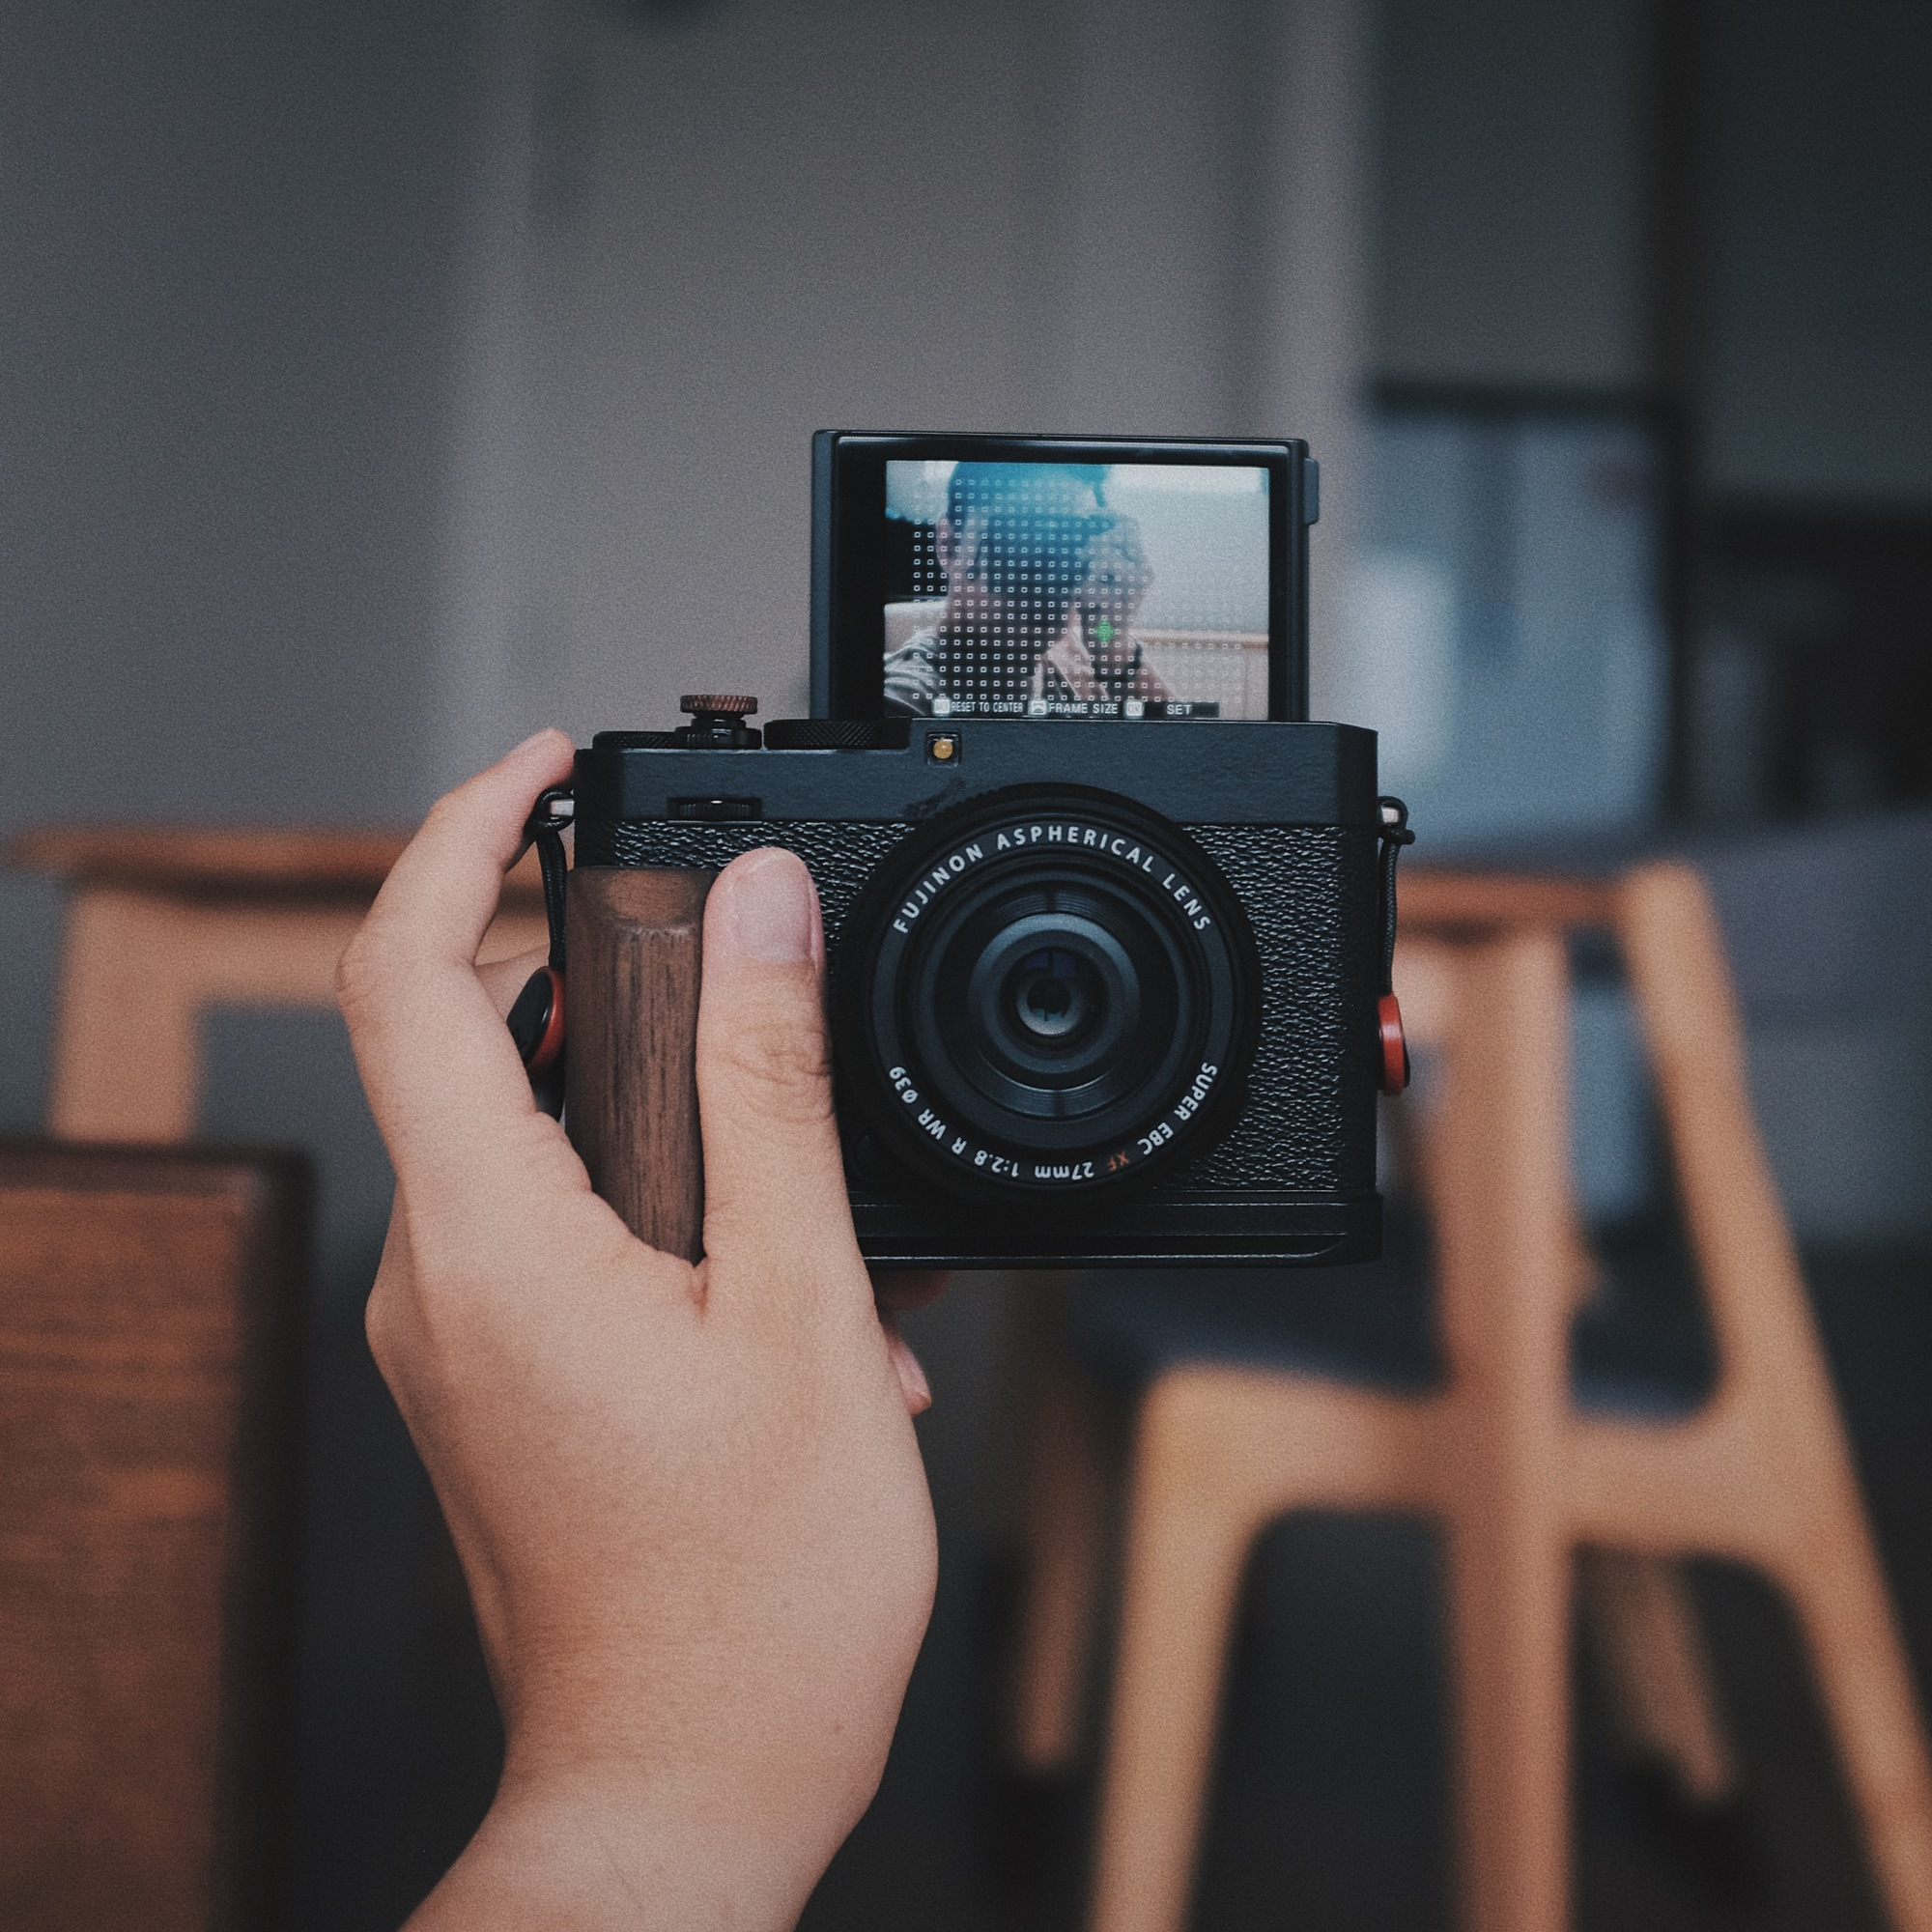
\includegraphics[width=\linewidth]{\envfinaldir/coverpic-prod.jpg}\par
            % \vskip 30pt
            \vfill

            \normalsize\rmfamily\scshape
            \copyright{} The Web Digest Project \hfill\large \envdatestr
        \end{center}
    \end{titlepage}
    % \restoregeometry
}
\newcommand{\simplehref}[1]{%
    \textcolor{blue!80!green}{\href{#1}{#1}}%
}
\renewcommand{\contentsname}{\center\Huge\sffamily\bfseries Contents\par\vskip 20pt}
\newcounter{ipartcounter}
\setcounter{ipartcounter}{0}
\newcommand{\ipart}[1]{
    % \vskip 20pt
    \clearpage
    \stepcounter{ipartcounter}
    \phantomsection
    \addcontentsline{toc}{chapter}{#1}
    % \begin{center}
    %     \Huge
    %     \sffamily\bfseries
    %     #1
    % \end{center}
    % \vskip 20pt plus 7pt
}
\newcounter{ichaptercounter}
\setcounter{ichaptercounter}{0}
\newcommand{\ichapter}[1]{
    % \vskip 20pt
    \clearpage
    \stepcounter{ichaptercounter}
    \phantomsection
    \addcontentsline{toc}{section}{\numberline{\arabic{ichaptercounter}}#1}
    \begin{center}
        \Huge
        \sffamily\bfseries
        #1
    \end{center}
    \vskip 20pt plus 7pt
}
\newcommand{\entrytitlefont}[1]{\subsection*{\raggedright\Large\sffamily\bfseries#1}}
\newcommand{\entryitemGeneric}[2]{
    % argv: title, url
    \parbox{\linewidth}{
        \entrytitlefont{#1}\par\vskip 5pt
        \footnotesize\ttfamily\mdseries
        \simplehref{#2}
    }\vskip 11pt plus 11pt minus 1pt
}
\newcommand{\entryitemGithub}[3]{
    % argv: title, url, desc
    \parbox{\linewidth}{
        \entrytitlefont{#1}\par\vskip 5pt
        \footnotesize\ttfamily\mdseries
        \simplehref{#2}\par\vskip 5pt
        \small\rmfamily\mdseries#3
    }\vskip 11pt plus 11pt minus 1pt
}
\newcommand{\entryitemAp}[3]{
    % argv: title, url, desc
    \parbox{\linewidth}{
        \entrytitlefont{#1}\par\vskip 5pt
        \footnotesize\ttfamily\mdseries
        \simplehref{#2}\par\vskip 5pt
        \small\rmfamily\mdseries#3
    }\vskip 11pt plus 11pt minus 1pt
}
\newcommand{\entryitemHackernews}[3]{
    % argv: title, hnurl, rawurl
    % \parbox{\linewidth}{
    %     \entrytitlefont{#1}\par\vskip 5pt
    %     \footnotesize\ttfamily\mdseries
    %     \simplehref{#3}\par
    %     \textcolor{black!50}{\href{#2}{#2}}
    % }\vskip 11pt plus 11pt minus 1pt
    \begin{minipage}{\linewidth}
            \entrytitlefont{#1}\par\vskip 5pt
            \footnotesize\ttfamily\mdseries
            \simplehref{#3}\par
            \textcolor{black!50}{\href{#2}{#2}}
    \end{minipage}\par\vskip 11pt plus 11pt minus 1pt
}







\begin{document}

\makeheader

\tableofcontents\clearpage




\ipart{Developers}
\ichapter{Hacker News}
\entryitemTwoLinks{Steam Brick: No screen, no controller, just a power button and a USB port}{https://news.ycombinator.com/item?id=42825441}{https://crastinator-pro.github.io/steam-brick/}

\entryitemTwoLinks{Larry Ellison: vast AI surveillance can ensure citizens are on best behavior (2024)}{https://news.ycombinator.com/item?id=42825097}{https://www.businessinsider.com/larry-ellison-ai-surveillance-keep-citizens-on-their-best-behavior-2024-9}

\entryitemTwoLinks{An invalid 68030 instruction accidentally allowed the Mac Classic II to boot}{https://news.ycombinator.com/item?id=42824562}{https://www.downtowndougbrown.com/2025/01/the-invalid-68030-instruction-that-accidentally-allowed-the-mac-classic-ii-to-successfully-boot-up/}

\entryitemTwoLinks{Wall Street banks prepare to sell up to \$3B in X loans next week}{https://news.ycombinator.com/item?id=42823908}{https://www.reuters.com/technology/wall-street-banks-set-sell-billions-dollars-x-loans-wsj-reports-2025-01-24/}

\entryitemTwoLinks{Every HTML Element}{https://news.ycombinator.com/item?id=42823722}{https://iamwillwang.com/dollar/every-html-element/}

\entryitemTwoLinks{OpenRA – Classic strategy games rebuilt for the modern era}{https://news.ycombinator.com/item?id=42823667}{https://www.openra.net/}

\entryitemTwoLinks{DeepSeek-R1: Incentivizing Reasoning Capability in LLMs via RL}{https://news.ycombinator.com/item?id=42823568}{https://arxiv.org/abs/2501.12948}

\entryitemTwoLinks{DOGE Takeover of USDS Allows Them to Surveil the US Government from the Inside}{https://news.ycombinator.com/item?id=42823510}{https://www.wired.com/story/doge-elon-musk/}

\entryitemTwoLinks{CIA now favors lab leak theory to explain Covid's origins}{https://news.ycombinator.com/item?id=42823385}{https://www.nytimes.com/2025/01/25/us/politics/cia-covid-lab-leak.html}

\entryitemTwoLinks{Doorbell camera catches rare footage of meteorite striking home's front walkway}{https://news.ycombinator.com/item?id=42821911}{https://www.cnn.com/2025/01/22/science/meteorite-strike-doorbell-camera/index.html}

\entryitemTwoLinks{Hacker infects 18,000 "script kiddies" with fake malware builder}{https://news.ycombinator.com/item?id=42821611}{https://www.bleepingcomputer.com/news/security/hacker-infects-18-000-script-kiddies-with-fake-malware-builder/}

\entryitemTwoLinks{Pixelfed Hit 500K Users}{https://news.ycombinator.com/item?id=42821519}{https://fedidb.org/software/pixelfed}

\entryitemTwoLinks{Show HN: I built a DIY plane spotting system at home}{https://news.ycombinator.com/item?id=42821457}{https://pilane.obviy.us/}

\entryitemTwoLinks{The Mythical IO-Bound Rails App}{https://news.ycombinator.com/item?id=42820419}{https://byroot.github.io/ruby/performance/2025/01/23/the-mythical-io-bound-rails-app.html}

\entryitemTwoLinks{First Look: Loops, by Pixelfed – Decentralised TikTok Competitor (2024)}{https://news.ycombinator.com/item?id=42820053}{https://wedistribute.org/2024/11/loops-early-look/}

\entryitemTwoLinks{TinyZero}{https://news.ycombinator.com/item?id=42819262}{https://github.com/Jiayi-Pan/TinyZero}

\entryitemTwoLinks{French police free kidnapped Ledger executive}{https://news.ycombinator.com/item?id=42819018}{https://moneycheck.com/french-police-free-kidnapped-ledger-executive-after-day-long-ordeal/}

\entryitemTwoLinks{Caltrain's electric fleet more efficient than expected}{https://news.ycombinator.com/item?id=42818692}{https://www.caltrain.com/news/caltrains-electric-fleet-more-efficient-expected}

\entryitemTwoLinks{File Explorer is merged to Helix editor}{https://news.ycombinator.com/item?id=42818278}{https://github.com/helix-editor/helix/pull/11285}

\entryitemTwoLinks{You could have invented Fenwick trees}{https://news.ycombinator.com/item?id=42818248}{https://www.cambridge.org/core/journals/journal-of-functional-programming/article/you-could-have-invented-fenwick-trees/B4628279D4E54229CED97249E96F721D}\ichapter{Phoronix}
\entryitemGeneric{\hskip 0pt{}Intel Media Driver 2024Q4 Released With Battlemage Video Encode}{https://www.phoronix.com/news/Intel-Media-Driver-2024Q4}

\entryitemGeneric{\hskip 0pt{}ISD: A New Interactive Way For systemd Management}{https://www.phoronix.com/news/ISD-Interactive-Systemd}

\entryitemGeneric{\hskip 0pt{}Much Faster Suspend \& Resume For Some Systems With Linux 6.14}{https://www.phoronix.com/news/Linux-6.14-ACPI}

\entryitemGeneric{\hskip 0pt{}Intel THC, Wacom PCI Device \& SteelSeries Arctis 9 Support Land In Linux 6.14}{https://www.phoronix.com/news/Linux-6.14-HID}

\entryitemGeneric{\hskip 0pt{}SUSE's New "Agama 11" Installer Preps For SLES 16 Beta / openSUSE Leap 16}{https://www.phoronix.com/news/SUSE-Agama-11-Installer}

\entryitemGeneric{\hskip 0pt{}Linux 6.14 Drops EFI's Long Obsolete UGA Protocol}{https://www.phoronix.com/news/Linux-6.14-EFI}

\entryitemGeneric{\hskip 0pt{}KDE Plasma 6.4 Begins Seeing Early Feature Work, Plasma 6.3 Sees More Fixes}{https://www.phoronix.com/news/KDE-Plasma-6.4-Starts}

\entryitemGeneric{\hskip 0pt{}Uncached Buffered I/O \& Some Other Nice Memory Management Optimizations With Linux 6.14}{https://www.phoronix.com/news/Linux-6.14-MM}

\entryitemGeneric{\hskip 0pt{}Linux 6.14 Adds Support For Blaize BLZP1600, SpacemiT K1 \& Snapdragon 8 Elite SoCs}{https://www.phoronix.com/news/Linux-6.14-SoCs}\ichapter{Dribbble}
\entryitemGeneric{\hskip 0pt{}Dyna - Logo Design}{https://dribbble.com/shots/25525428-Dyna-Logo-Design}

\entryitemGeneric{\hskip 0pt{}Godzilla Logo}{https://dribbble.com/shots/25525727-Godzilla-Logo}

\entryitemGeneric{\hskip 0pt{}B}{https://dribbble.com/shots/25524895-B}

\entryitemGeneric{\hskip 0pt{}Tattooed Devil Horns}{https://dribbble.com/shots/25520911-Tattooed-Devil-Horns}

\entryitemGeneric{\hskip 0pt{}Carbon Solutions B2B Dashboard Design}{https://dribbble.com/shots/25506638-Carbon-Solutions-B2B-Dashboard-Design}

\entryitemGeneric{\hskip 0pt{}Goose Gym}{https://dribbble.com/shots/25515121-Goose-Gym}

\entryitemGeneric{\hskip 0pt{}HappyDev - Logo Design / Branding}{https://dribbble.com/shots/25514894-HappyDev-Logo-Design-Branding}

\entryitemGeneric{\hskip 0pt{}VCC Unused Logo Design Concept}{https://dribbble.com/shots/25511334-VCC-Unused-Logo-Design-Concept}

\entryitemGeneric{\hskip 0pt{}Rapid Rabbit Logo}{https://dribbble.com/shots/25516738-Rapid-Rabbit-Logo}

\entryitemGeneric{\hskip 0pt{}Product design - icons set}{https://dribbble.com/shots/25516253-Product-design-icons-set}

\entryitemGeneric{\hskip 0pt{}The Toucan}{https://dribbble.com/shots/25515890-The-Toucan}

\entryitemGeneric{\hskip 0pt{}LLM GPU Manager}{https://dribbble.com/shots/25513811-LLM-GPU-Manager}

\entryitemGeneric{\hskip 0pt{}Bestest Brand®}{https://dribbble.com/shots/25510300-Bestest-Brand}

\entryitemGeneric{\hskip 0pt{}QVELTY / Design \& Animation}{https://dribbble.com/shots/25507639-QVELTY-Design-Animation}

\entryitemGeneric{\hskip 0pt{}Wine Label}{https://dribbble.com/shots/25509757-Wine-Label}

\entryitemGeneric{\hskip 0pt{}Haptic Logo Design}{https://dribbble.com/shots/25504012-Haptic-Logo-Design}

\entryitemGeneric{\hskip 0pt{}Letter V + LED + Wires Logo}{https://dribbble.com/shots/25507506-Letter-V-LED-Wires-Logo}

\entryitemGeneric{\hskip 0pt{}Robin bird logo}{https://dribbble.com/shots/25509208-Robin-bird-logo}

\entryitemGeneric{\hskip 0pt{}Qore - Logo Design}{https://dribbble.com/shots/25509466-Qore-Logo-Design}

\entryitemGeneric{\hskip 0pt{}Wine Label}{https://dribbble.com/shots/25503830-Wine-Label}

\entryitemGeneric{\hskip 0pt{}Monocle Cat}{https://dribbble.com/shots/25502155-Monocle-Cat}

\entryitemGeneric{\hskip 0pt{}Roundrobin}{https://dribbble.com/shots/25502404-Roundrobin}

\entryitemGeneric{\hskip 0pt{}Mobile Game Design}{https://dribbble.com/shots/25498605-Mobile-Game-Design}

\entryitemGeneric{\hskip 0pt{}Fitness App Design}{https://dribbble.com/shots/25494068-Fitness-App-Design}


\ipart{Developers~~~~(zh-Hans)}
\ichapter{Solidot}
\entryitemGeneric{\hskip 0pt{}巴基斯坦议会通过法案全面控制社交媒体}{https://www.solidot.org/story?sid=80423}

\entryitemGeneric{\hskip 0pt{}AI 犯的错误和人类不同}{https://www.solidot.org/story?sid=80422}

\entryitemGeneric{\hskip 0pt{}数百超级富豪呼吁对其征收更高的税}{https://www.solidot.org/story?sid=80421}

\entryitemGeneric{\hskip 0pt{}Linux 6.14 加入对微软 Copilot 按键的支持}{https://www.solidot.org/story?sid=80420}

\entryitemGeneric{\hskip 0pt{}秘密后门使用``魔法封包''感染企业 VPN}{https://www.solidot.org/story?sid=80419}

\entryitemGeneric{\hskip 0pt{}调查显示八成游戏开发商开发 PC 游戏}{https://www.solidot.org/story?sid=80418}

\entryitemGeneric{\hskip 0pt{}《自然》调查显示七成回应者使用 Bluesky}{https://www.solidot.org/story?sid=80417}

\entryitemGeneric{\hskip 0pt{}乔治 R.R.马丁合作发表了一篇物理学论文}{https://www.solidot.org/story?sid=80416}

\entryitemGeneric{\hskip 0pt{}Google 移动搜索移除网址面包屑导航}{https://www.solidot.org/story?sid=80415}

\entryitemGeneric{\hskip 0pt{}癌细胞利用有缺陷的线粒体毒害攻击免疫细胞}{https://www.solidot.org/story?sid=80414}

\entryitemGeneric{\hskip 0pt{}日本市场中国平板电视首次超过五成}{https://www.solidot.org/story?sid=80413}

\entryitemGeneric{\hskip 0pt{}智人离开非洲后血型可能发生适应性遗传变化}{https://www.solidot.org/story?sid=80412}

\entryitemGeneric{\hskip 0pt{}三菱不打算参与本田日产的合并}{https://www.solidot.org/story?sid=80411}

\entryitemGeneric{\hskip 0pt{}特朗普政府暂停了 NIH 的会议和旅行}{https://www.solidot.org/story?sid=80410}

\entryitemGeneric{\hskip 0pt{}Debian 15 代号 Duke}{https://www.solidot.org/story?sid=80409}

\entryitemGeneric{\hskip 0pt{}研究揭示不同政治光谱对传递虚假信息的偏好}{https://www.solidot.org/story?sid=80408}

\entryitemGeneric{\hskip 0pt{}万事达卡 DNS 错误存在了五年之久}{https://www.solidot.org/story?sid=80405}

\entryitemGeneric{\hskip 0pt{}Debian 13.0 Trixie 预计今年夏天发布}{https://www.solidot.org/story?sid=80404}

\entryitemGeneric{\hskip 0pt{}Telegram 屏蔽 RuTracker 频道}{https://www.solidot.org/story?sid=80402}

\entryitemGeneric{\hskip 0pt{}在出售给美国买家前苹果应用商店不会重新上架 TikTok}{https://www.solidot.org/story?sid=80400}\ichapter{V2EX}
\entryitemGeneric{\hskip 0pt{}[ WATCH] Apple Watch 睡眠监测不准}{https://www.v2ex.com/t/1107875}

\entryitemGeneric{\hskip 0pt{}[问与答] 大家用 cursor 的时候,怎么解决回复可能不可靠的问题?}{https://www.v2ex.com/t/1107874}

\entryitemGeneric{\hskip 0pt{}[程序员] dokploy 如何部署 nuxt 项目?(进来少踩坑)}{https://www.v2ex.com/t/1107873}

\entryitemGeneric{\hskip 0pt{}[职场话题] 高校合同工值得去么?}{https://www.v2ex.com/t/1107872}

\entryitemGeneric{\hskip 0pt{}[Apple] 到现在还没有一个行情软件支持实时活动和灵动岛吗}{https://www.v2ex.com/t/1107871}

\entryitemGeneric{\hskip 0pt{}[Apple] 国内 JCB 信用卡均已经无法绑定日区 Apple ID}{https://www.v2ex.com/t/1107870}

\entryitemGeneric{\hskip 0pt{}[问与答] v2exer 可以放烟花吗,价格如何}{https://www.v2ex.com/t/1107869}

\entryitemGeneric{\hskip 0pt{}[广州] 广州今年过年有没有可以上门喂猫的,主要是陪玩一下。市场价结算}{https://www.v2ex.com/t/1107868}

\entryitemGeneric{\hskip 0pt{}[分享发现] Anki 使用经验贴}{https://www.v2ex.com/t/1107867}

\entryitemGeneric{\hskip 0pt{}[分享创造] TabTab - Cursor / Trae 帮我写的第一个浏览器插件}{https://www.v2ex.com/t/1107866}

\entryitemGeneric{\hskip 0pt{}[公司运营] 大家跟客户报价的时候会报两个价格吗,走公司户/个人户}{https://www.v2ex.com/t/1107864}

\entryitemGeneric{\hskip 0pt{}[iPad] 想买个 mini7 咋这么难?}{https://www.v2ex.com/t/1107863}

\entryitemGeneric{\hskip 0pt{}[宽带症候群] 光猫改桥接后改 ip 地址,脑抽改成 192.168.5.255}{https://www.v2ex.com/t/1107862}

\entryitemGeneric{\hskip 0pt{}[Los Angeles] 有没有在加州的朋友,闲来无事,做了一个华人网}{https://www.v2ex.com/t/1107861}

\entryitemGeneric{\hskip 0pt{}[C++] 有没有合适开源的 C++项目可以快速实现一些功能}{https://www.v2ex.com/t/1107860}

\entryitemGeneric{\hskip 0pt{}[香港] 高德接入香港打车了,过来玩如果不方便安装 uber 且不想打出租,可以试试。}{https://www.v2ex.com/t/1107859}

\entryitemGeneric{\hskip 0pt{}[问与答] v 友们,帮忙看一下我是不是买到假茶叶了}{https://www.v2ex.com/t/1107858}

\entryitemGeneric{\hskip 0pt{}[问与答] 为什么我的 win10 这么卡}{https://www.v2ex.com/t/1107857}

\entryitemGeneric{\hskip 0pt{}[宽带症候群] 据 DMIT 的消息, LAX Pro v6 不使用 AS4809 的 CN2,居然是境内段 CN 2 没有完成 IPv6 的网络建设?}{https://www.v2ex.com/t/1107856}

\entryitemGeneric{\hskip 0pt{}[问与答] Windows 有没有程序可以修改任务栏中任意程序的托盘图标?}{https://www.v2ex.com/t/1107855}

\entryitemGeneric{\hskip 0pt{}[Mac mini] 买 Mac 电脑,一定要把所有预算堆到内存上,一定一定记住。}{https://www.v2ex.com/t/1107853}

\entryitemGeneric{\hskip 0pt{}[宽带症候群] 新房子網絡設備全移動,求破局方式}{https://www.v2ex.com/t/1107850}

\entryitemGeneric{\hskip 0pt{}[问与答] 肯尼迪事件解密了,凶手是谁?}{https://www.v2ex.com/t/1107849}

\entryitemGeneric{\hskip 0pt{}[分享创造] 还在为思维混乱发愁?这款神器帮你一键梳理!}{https://www.v2ex.com/t/1107846}

\entryitemGeneric{\hskip 0pt{}[职场话题] 大家对 b 端, c 端的英文词汇一般用什么来表达}{https://www.v2ex.com/t/1107845}

\entryitemGeneric{\hskip 0pt{}[Apple] 快过年发现被妹妹和苹果联合爆金币了}{https://www.v2ex.com/t/1107844}

\entryitemGeneric{\hskip 0pt{}[问与答] 第一次参加不怎么熟悉的人的婚礼,应该去注意什么。}{https://www.v2ex.com/t/1107842}

\entryitemGeneric{\hskip 0pt{}[问与答] 目前找工作最好的方式是?}{https://www.v2ex.com/t/1107840}

\entryitemGeneric{\hskip 0pt{}[宽带症候群] 四川移动宽带,烽火 HG5043F 光猫改桥接和 IPV6,神奇方法与疑问}{https://www.v2ex.com/t/1107839}

\entryitemGeneric{\hskip 0pt{}[Local LLM] 🦙 对话效果最好的 7B/1.5B 模型大家用的哪个?}{https://www.v2ex.com/t/1107837}

\entryitemGeneric{\hskip 0pt{}[macOS] mac screen sharing app 使用高性能模式连接另一个 mac 在使用 surge ponte 情况下 不可用}{https://www.v2ex.com/t/1107835}

\entryitemGeneric{\hskip 0pt{}[问与答] 指数估值哪家准}{https://www.v2ex.com/t/1107834}

\entryitemGeneric{\hskip 0pt{}[深圳] 深圳南山租房求推荐}{https://www.v2ex.com/t/1107833}

\entryitemGeneric{\hskip 0pt{}[职场话题] 新年快乐!远程办公,想给国外同事发礼物,发什么好呢?}{https://www.v2ex.com/t/1107832}

\entryitemGeneric{\hskip 0pt{}[问与答] 如何整治小区里没素质的人?}{https://www.v2ex.com/t/1107831}

\entryitemGeneric{\hskip 0pt{}[问与答] Windows 会自动同步 WIFI 密码吗?}{https://www.v2ex.com/t/1107830}

\entryitemGeneric{\hskip 0pt{}[投资] 2024 年我在 A 股赚了 20 万}{https://www.v2ex.com/t/1107829}

\entryitemGeneric{\hskip 0pt{}[前端开发] 一个后端开发想学前端开发我究竟该学哪些东西?}{https://www.v2ex.com/t/1107828}

\entryitemGeneric{\hskip 0pt{}[职场话题] 28 岁转码建议?}{https://www.v2ex.com/t/1107827}

\entryitemGeneric{\hskip 0pt{}[分享发现] 12306 相比第三方的缺点}{https://www.v2ex.com/t/1107826}

\entryitemGeneric{\hskip 0pt{}[Apple] macOS 的 WindowServer 的 GPU 占用率高的问题?}{https://www.v2ex.com/t/1107825}

\entryitemGeneric{\hskip 0pt{}[前端开发] 前端问题求助}{https://www.v2ex.com/t/1107824}

\entryitemGeneric{\hskip 0pt{}[Android] 有什么类似 RePlugin 这种,能在 APK 中运行 APK 的框架}{https://www.v2ex.com/t/1107823}

\entryitemGeneric{\hskip 0pt{}[音乐] 原道的入耳系列的 ``有线动圈入耳式耳机'' 音质效果还没有老版本的好}{https://www.v2ex.com/t/1107822}

\entryitemGeneric{\hskip 0pt{}[问与答] AMD:已将 DeepSeek-V3 模型集成到 Instinct MI300X GPU 上,利用 SGLang 彻底改变 AI 开发}{https://www.v2ex.com/t/1107820}

\entryitemGeneric{\hskip 0pt{}[汽车] 小型纯电车怎么选五菱缤果还是吉利星愿?}{https://www.v2ex.com/t/1107819}

\entryitemGeneric{\hskip 0pt{}[分享发现] 懒人日记党狂喜,用卡片的方式写日记🥰}{https://www.v2ex.com/t/1107816}

\entryitemGeneric{\hskip 0pt{}[分享创造] [Local Dream] 在 Android 端运行 Stable Diffusion,支持骁龙 NPU 加速}{https://www.v2ex.com/t/1107815}

\entryitemGeneric{\hskip 0pt{}[分享创造] 做一个小工具来练手 AI 开发}{https://www.v2ex.com/t/1107814}

\entryitemGeneric{\hskip 0pt{}[iOS] iOS 中有没有支持连续复制的剪贴板软件?}{https://www.v2ex.com/t/1107813}


\ipart{Generic News}







\clearpage
\leavevmode\vfill
\footnotesize

Copyright \copyright{} 2023-2025 Neruthes and other contributors.

This document is published with CC BY-NC-ND 4.0 license.

The entries listed in this newsletter may be copyrighted by their respective creators.

This newsletter is generated by the Web Digest project.

The newsletters are also delivered via Telegram channel \CJKunderline{\href{https://t.me/webdigestchannel}{https://t.me/webdigestchannel}}.\\
RSS feed is available at \CJKunderline{\href{https://webdigest.pages.dev/rss.xml}{https://webdigest.pages.dev/rss.xml}}.

This newsletter is available in PDF at
\CJKunderline{\href{https://webdigest.pages.dev/}{https://webdigest.pages.dev/}}.

The source code being used to generate this newsletter is available at\\
\CJKunderline{\href{https://github.com/neruthes/webdigest}{https://github.com/neruthes/webdigest}}.

This newsletter is also available in
\CJKunderline{\href{http://webdigest.pages.dev/readhtml/\envyear/WebDigest-20250126.html}{HTML}} and
\CJKunderline{\href{https://github.com/neruthes/webdigest/blob/master/markdown/\envyear/WebDigest-20250126.md}{Markdown}}.


\coverpic{https://unsplash.com/photos/an-exit-sign-is-seen-through-a-window-6zKl5S7sqXs}{Macy Taylor}


\end{document}
